\documentclass[tikz,border=10pt]{standalone}
\begin{document}
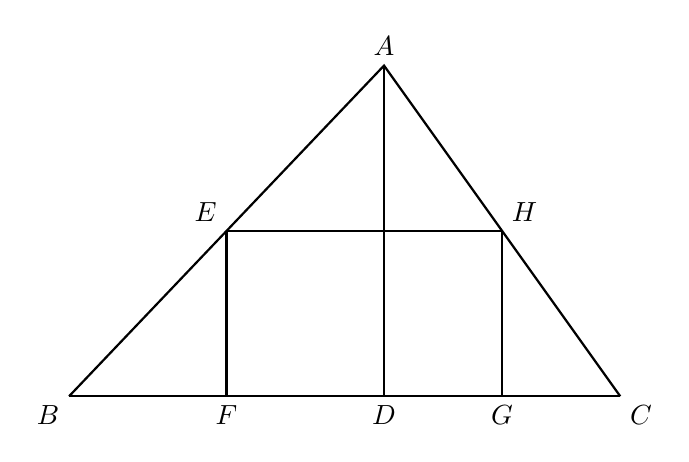
\begin{tikzpicture}
  \coordinate (B) at (0,0);
  \coordinate (C) at (7,0);
  \coordinate (D) at (4,0);
  \coordinate (A) at (4,4.2);
  \coordinate (E) at (2,2.1);
  \coordinate (H) at (5.5,2.1);
  \coordinate (F) at (2,0);
  \coordinate (G) at (5.5,0);

  \draw[thick] (B) -- (C);
  \draw[thick] (B) -- (A) -- (C);
  \draw[thick] (A) -- (D);
  \draw[thick] (E) -- (H);
  \draw[thick] (E) -- (F);
  \draw[thick] (H) -- (G);

  \node[above] at (A) {$A$};
  \node[below left] at (B) {$B$};
  \node[below right] at (C) {$C$};
  \node[below] at (D) {$D$};
  \node[above left] at (E) {$E$};
  \node[above right] at (H) {$H$};
  \node[below] at (F) {$F$};
  \node[below] at (G) {$G$};
\end{tikzpicture}
\end{document}
